\documentclass[12pt, a4paper]{article}

\usepackage[czech]{babel}
\usepackage{lmodern}
\usepackage[utf8]{inputenc}
\usepackage[T1]{fontenc}
\usepackage[pdftex]{graphicx}
\usepackage{amsmath}
\usepackage[hidelinks,unicode]{hyperref}
\usepackage{float}
\usepackage{listings}
\usepackage{tikz}
\usepackage{xcolor}
\usepackage{tabularx}
\usepackage[final]{pdfpages}
\usepackage{syntax}


\definecolor{mauve}{rgb}{0.58,0,0.82}
\usetikzlibrary{shapes,positioning,matrix,arrows}

\newcommand{\img}[1]{(viz obr. \ref{#1})}

\definecolor{pblue}{rgb}{0.13,0.13,1}
\definecolor{pgreen}{rgb}{0,0.5,0}
\definecolor{pred}{rgb}{0.9,0,0}
\definecolor{pgrey}{rgb}{0.46,0.45,0.48}


\lstdefinestyle{flex}{
    frame=tb,
    aboveskip=3mm,
    belowskip=3mm,
    showstringspaces=false,
    columns=flexible,
    basicstyle={\small\ttfamily},
    numbers=none,
    numberstyle=\tiny\color{black},
    keywordstyle=\color{black},
    commentstyle=\color{black},
    stringstyle=\color{black},
    breaklines=true,
    breakatwhitespace=true,
    tabsize=3
}

\lstset{
    frame=tb,
    language=C,
    aboveskip=3mm,
    belowskip=3mm,
    showstringspaces=false,
    columns=flexible,
    basicstyle={\small\ttfamily},
    numbers=none,
    numberstyle=\tiny\color{gray},
    keywordstyle=\color{blue},
    commentstyle=\color{pgreen},
    stringstyle=\color{mauve},
    breaklines=true,
    breakatwhitespace=true,
    tabsize=3
}


\let\oldsection\section
\renewcommand\section{\clearpage\oldsection}

\begin{document}
	% this has to be placed here, after document has been created
	% \counterwithout{lstlisting}{chapter}
	\renewcommand{\lstlistingname}{Ukázka kódu}
	\renewcommand{\lstlistlistingname}{Seznam ukázek kódu}
    \begin{titlepage}

        \centering

        \vspace*{\baselineskip}
        \begin{figure}[H]
        \centering
        
\includegraphics[width=7cm]{img/fav-logo.jpg}
        \end{figure}

        \vspace*{1\baselineskip}

        \vspace{0.75\baselineskip}

        \vspace{0.5\baselineskip}
        {Semestrální práce z předmětu KIV/FJP}

        {\LARGE\sc Tvorba vlastního překladače\\}
        {\sc pro vlastní jazyk C-{}-\\}

        \vspace{4\baselineskip}

        \vspace{0.5\baselineskip}

        {\sc\Large Jindřiška Reismüllerová \\}
        \vspace{0.5\baselineskip}
        {A20N0061P}

        {\sc\Large Stanislav Král \\}
        \vspace{0.5\baselineskip}
        {A20N0091P}

        \vfill

        {\sc Západočeská univerzita v Plzni\\
        Fakulta aplikovaných věd}

    \end{titlepage}


    % TOC
    \tableofcontents
    \pagebreak

    
\section{Zadání}

    Cílem práce je vytvořit překladač zvoleného jazyka, kdy je možné se inspirovat jazykem PL/0, vybrat si podmožninu nnějakého existujícího jazyka nebo si navrhnout jazyk zcela vlastní. Cílová architektura je volitelná, avšak nesmí být použit vlastní interpret.


\section{Návrh vlastního jazyka}

V rámci této semestrální práce byl navržen jednoduchý jazyk C-{}- (\textit{C minus minus}), který vychází z jazyka C a podporuje podmnožinu jeho konstrukcí.

\begin{lstlisting}[caption={Ukázka programu v jazyce C-{}-}, captionpos=b]
int main() {
    i int;
    j int = 0;

    for (i = 0; i < 10; i = i + 1) {
        j = j + i;
    }

    return 0;
}
\end{lstlisting}


\subsection{Specifikace typu a názvu proměnné}
Po vzoru moderních jazyků typu Kotlin, Go nebo např. Rust, navržený jazyk používá opačné pořadí slov při deklaraci názvu a typu proměnné. 

Hlavní myšlenkou tohoto způsobu deklarace proměnné je snaha, aby programátoři kladli větší důraz na názvy používaných proměnných -- před specifikací typu je třeba se zamyslet nad jejím názvem. 

\subsection{Absence operátorů \texttt{++} a \texttt{-{}-}}

Podobně, jako například jazyk Python, navržený jazyk C-{}- nepodporuje operátory \texttt{++} a \texttt{-{}-}. Toto rozhodnutí bylo učiněno pouze z důvodu odlišení od jazyka C, z kterého navržený jazyk vychází.

\subsection{Gramatika jazyka}
% TODO
\begin{grammar}

<statement> ::= <ident> `=' <expr> 
\alt `for' <ident> `=' <expr> `to' <expr> `do' <statement> 
\alt `{' <stat-list> `}' 
\alt <empty> 

<stat-list> ::= <statement> `;' <stat-list> | <statement> 

\end{grammar}




\section{Návrh architektury překladače}

\subsection{Výběr programovacího jazyka}
\subsubsection{Haskell}
Při výběru technologií pro vytvoření překladače navrženého jazyka připadal nejdřív v úvahu jazyk Haskell, který je pro tvorbu překladačů často používán hlavně kvůli tomu, že se jedná o funkcionální jazyk, a definice různých přepisovacích pravidel či zpracování vstupního textu je tak velmi jednoduchá a přirozená. Další velkou výhodou je existence knihovny \texttt{Parsec}\footnote{\url{https://hackage.haskell.org/package/parsec}} vytvořené pro tento jazyk, která je velmi kvalitní a vhodná pro lexikální analýzu.

 Avšak z důvodu velké odlišnosti Haskellu od běžně používaných programovacích jazyků, kdy Haskell používá spoustu fundamentálně odlišných konstrukcí pro zápis programů, bylo nakonec od možnosti využít tento programovací jazyk odstopueno.
 
\subsubsection{C a C++}
Jako další vhodná možnost se jevil výběr použití kombinace jazyků C a C++, které spolu s použitím knihovnen \texttt{bison}\footnote{\url{https://github.com/akimd/bison}} a \texttt{flex}\footnote{\url{https://github.com/westes/flex}} poskytují pevný základ pro tvorbu překladačů, a existuje velké množství literatury či článků pokrývající tuto problmatiku.

Tato kombinace byla nakonec vybrána jako náhrada za zavrhnutý jazyk Haskell.


\subsection{Lexikální analyzátor}

K převodu proudu znaků zdrojového kódu na proud tokenů, které představují logické jednotky programu, je třeba navrhnout a implementovat lexikální analyzátor. 

Jednotlivé tokeny jsou popsány regulárními výrazy, jež jsou dále implementovány pomocí deterministikých konečných automatů. Ke každému tokenu je také třeba i uchovávat lexém, který představuje terminální symbol jazyka.

\newpage
Seznam tokenů vyhledávaných během lexikální analýzy při překladu zdrojového kódu v jazyce C-{}-:

\begin{itemize}
    \item \textbf{klíčová slova} -- \texttt{STRUCT}, \texttt{WHILE}, \texttt{FOR}, \texttt{IF}, \texttt{ELSE}, \texttt{CONST}, \texttt{RETURN}, \texttt{TRUE}, \texttt{FALSE}

    \item \textbf{aritmetické a logické operátory} -- \texttt{L\_OP}, \texttt{B\_OP}, \texttt{A\_OP}, \texttt{COMPARSION}, \texttt{NOT}
    \item \textbf{závorky} -- \texttt{B\_L\_CURLY}, \texttt{B\_R\_CURLY}, \texttt{B\_L\_SQUARE}, \texttt{B\_R\_SQUARE}, \texttt{PAREN\_L}, \texttt{PAREN\_R}
    \item \textbf{ostatní} -- \texttt{TYPE}, \texttt{IDENTIFIER}, \texttt{STR\_LITERAL}, \texttt{INT\_LITERAL}, \texttt{SEMICOLON}, \texttt{COMMA}, \texttt{DOT}, \texttt{ASSIGN}, \texttt{OTHER}


\end{itemize}

V rámci této semestrální práce byl pro implementaci lexikálního analyzátoru použit nástroj \texttt{lex}, který pro tokeny definované regulárními výrazy vygeneruje kód v programovacím jazyce C. Tento kód představuje implementaci deterministického konečného automatu.

\begin{lstlisting}[caption={Ukázka regulárních výrazů pro skenování tokenů}, captionpos=b, style=flex]
type            (int|string|char|bool)
identifier      ([a-z][a-zA-Z0-9]*)
int_literal     ([0-9])+
str_literal     \"(\\.|[^"\\])*\"
l_op            (\|\||\&\&)
b_op            (\||\&|\~)
a_op            (\+|\*|\/|\-)
comparsion      (>|<|==|>=|<=|!=)
\end{lstlisting}

\subsection{Syntaktická analýza}

Během syntaktické analýzy se typicky zpracovává vstupní text, který se nejčastěji transformuje na syntaktický strom, abstraktní derivační strom nebo jiné definované struktury. Pro zjednodušení této transformace se místo prostého vstupního textu zpracovává proud tokenů generován lexikální analýzou.

Smyslem syntaktické analýzy je zkoumat posloupnost tokenů a vyhodnotit, zdali vstupní text patří do daného programovacího jazyka definovaného gramatikou.

Pro implementaci syntaktického analyzátoru v této semestrální práci jsme zvolili nástroj \texttt{bison}, který umožňuje definovat gramatiku v Backus–Naurově formě.

\begin{lstlisting}[caption={Ukázka pravidla v \texttt{bison} syntaxi pro deklaraci proměnné}, captionpos=b, style=flex]
declaration:
    TYPE IDENTIFIER {
        printf("variable declaration: type=%d identifier=%s\n", $1, $2);
        $$ = new declaration($1, $2);
    }
\end{lstlisting}


\subsection{Abstraktní syntaktický strom}

Aby bylo možné generovat kód či instrukce překládaného zdrojového kódu do cílové platformy, je třeba sestavit abstraktní syntaktický strom. Po úspěšném sestavení probíhá jeho vyhodnocení, při kterém je generován kód či instrukce cílové platformy.

\begin{figure}[!ht]
    \centering
    {\includegraphics[width=\textwidth]{pdf/syntanalysis2.pdf}}
    \caption{Abstraktní syntaktický strom}
    \label{fig:screen-transition-diagram}
\end{figure}

Generování abstraktního syntaktického stromu probíhá během zpracovávání tokenů během syntaktické analýzy. 


\begin{figure}[!ht]
    \centering
    {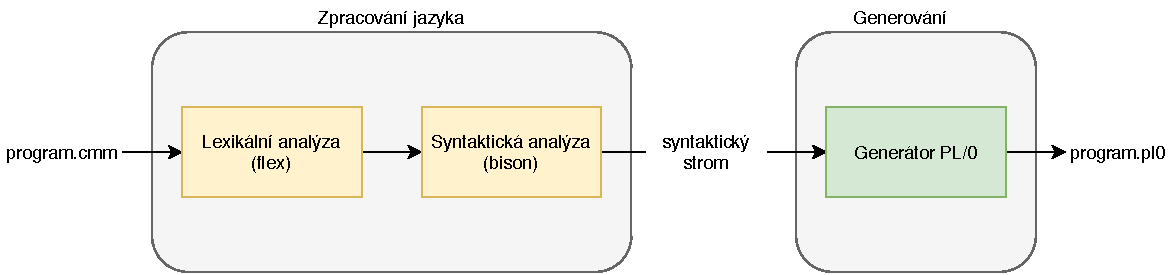
\includegraphics[width=\textwidth]{pdf/architecture.pdf}}
    \caption{Architektura překladače}
    \label{fig:screen-transition-diagram}
\end{figure}

\section{Závěr}	

% TODO

\end{document}    
